%===================================================================================================
\subsection{Preliminaries}\label{mod.par.math}
%---------------------------------------------------------------------------------------------------
\paragraph{Deriving Prior Distributions}
Uncertainty distributions for most parameters and calibration targets were estimated by
fitting a parametric distribution to specified quantiles.
Let $f\,(x\mid\theta)$ be
the probability density function of random variable~$x$ (parameter or calibration target)
given distribution parameters $\theta$.
Then $F\,(x\mid\theta) = \int_0^x f(\tau)\,d\tau$ is the cumulative distribution function,
and $Q(p\mid\theta) = F^{\,-1}(p\mid\theta)$ is the quantile function.
Our objective is to estimate $\theta$, given a set of quantiles
(\eg $q = \{q_{2.5},q_{97.5}\}$ for the 95\%~CI).
For each estimation, we minimized the following error function,
using the L-BFGS-B algorithm \cite{Byrd1995}:
\begin{equation}
  J(\theta) = \sum_i {\big|\,q_i - Q(p_i\mid\theta)\,\big|}^{\,\omega}
\end{equation}
where $\omega$ can specify absolute differences ($\omega=1$) or squared differences ($\omega=2$)
to improve convergence.
Distribution fit was validated visually using a plot of
the distribution quantiles $Q(p_i\mid\theta)$ \vs the target quantiles $q_i$,
overlaid on the density distribution $f\,(x\mid\theta)$; \eg Figure~\ref{fig:distr.fit}.
\begin{figure}[h]
  \centering
  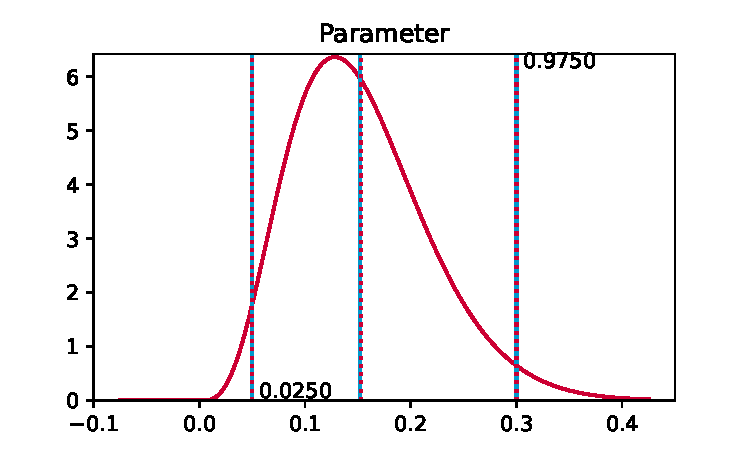
\includegraphics[width=.6\linewidth]{distr.fit}
  \caption{Example distribution fitting validation plot}
  \label{fig:distr.fit}
  \floatfoot{BAB distribution fit to $\{q_{2.5} = .05, q_{97.5} = .30\}$;
    blue solid lines: target quantiles $q_i$;
    red dotted lines: distribution quantiles $Q(p_i\mid\theta)$;
    red solid line: density distribution $f\,(x\mid\theta)$.}
\end{figure}
%---------------------------------------------------------------------------------------------------
\paragraph{Beta Approximation of the Binomial (BAB) Distribution}
Numerous model parameters and calibration targets represent population proportions.
Such proportions can be estimated as $\rho = n / N$, where
$N$ is the sample size and $n$ is the number of individuals with the characteristic of interest.
The uncertainty around $n$ is then given by the binomial distribution:
\begin{equation}\label{eq:binom}
  p(n) = {N \choose n} \, \rho^{n}{(1 - \rho)}^{N - n}
\end{equation}
However, \eqref{eq:binom} is only defined for discrete values of $n$.
It is more convenient to have a continuous distribution for $\rho$,
for sampling parameters and evaluating the likelihood of calibration targets,
since compartmental models can have non-whole-number population sizes.
For this purpose, we use a beta approximation of the binomial distribution (BAB):
\begin{equation}\label{eq:beta}
  p(\rho) =
    \frac{\Gamma(\alpha+\beta)}{\Gamma(\alpha)\,\Gamma(\beta)}\,
    \rho^{\alpha-1}{(1 - \rho)}^{\beta-1}
\end{equation}
with $\alpha = N\,\rho$ and $\beta = N\,(1-\rho)$.
Unlike the approximation by a normal distribution,
the beta distribution ensures that $\rho \in [0,1]$.
Figure~\ref{fig:bab} illustrates the approximation for
$N = \{10,20,40\}$ and $\rho = \{0.01,0.1,0.5\}$.
\begin{figure}
  \centering
  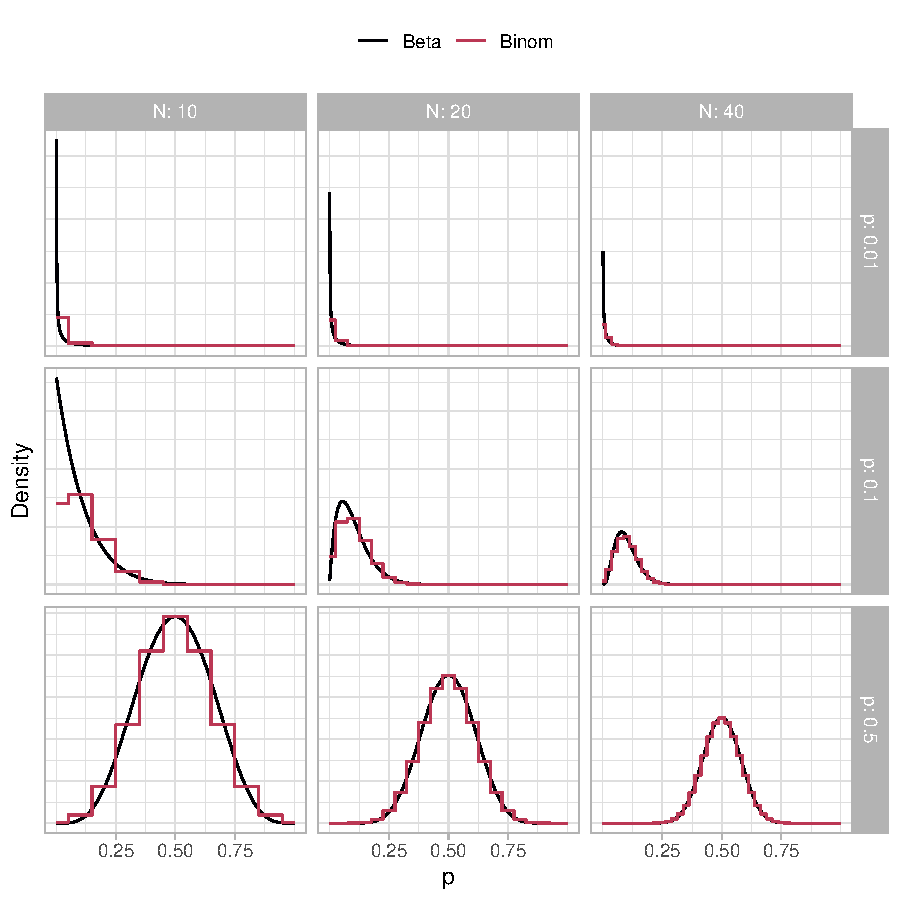
\includegraphics[width=.8\linewidth]{bab}
  \caption{Beta approximation of the binomial distribution (BAB)}
  \label{fig:bab}
\end{figure}
